\documentclass[math,code]{amznotes}
\setcounter{tocdepth}{2}  % Only show sections in the ToC
\usepackage[utf8]{inputenc}
\usepackage{amsmath}
\usepackage{amsfonts}
\usepackage{graphicx}
\usepackage{tikz}
\usepackage{etoolbox}
\usepackage{tabularx}
\usepackage{float} % Needed for [H] placement specifier
\usepackage{wrapfig} % Needed for wrapping figures

\graphicspath{ {./images/} }
\geometry{
    a4paper,
    headheight = 1.5cm
}

\patchcmd{\chapter}{\thispagestyle{plain}}{\thispagestyle{fancy}}{}{}

\theoremstyle{remark}
\newtheorem*{claim}{Claim}
\newtheorem*{remark}{Remark}
\newtheorem{case}{Case}

\begin{document}
\fancyhead[L]{
    Differential Equations for Engineering
}
\fancyhead[R]{
    Lecture Notes
}
\tableofcontents

\chapter{The Harmonic Oscillator}
\section{Simple Harmonic Motion}
\subsection{Damped Oscillations}
In the real world, oscillations seldom follow true SHM. Friction of some sort usually acts to dampen the motion so it dies away.

To analyze a system with damped oscillations. Let's assume the damping force is proportional to the velocity and acts against the direction of motion ($F_D=-b$). The net force on the mass is therefore:
\begin{equation}
    ma=-bv-kx
\end{equation}
Writing this as a differential equation in x, we obtain
\begin{align}
    m\ddot{x}=-b\dot{x}-kx \\
    m\ddot{x}+b\dot{x}+kx=0
\end{align}
To determine the solution for this differential equation, let's use the method of characterization equation. Firstly, form our characterization equation
\begin{equation}
    \lambda^2+\frac{b}{m}\lambda+\frac{k}{m}=0
\end{equation}
where its discriminant $\Delta=\frac{b^2}{m^2}-\frac{4k}{m}$. And based on this $\Delta$, we have the following three cases of solution
\begin{enumerate}
    \item If $\Delta<0\text{ or, }b^2<4mk$, we have complex conjugate roots $\lambda=\alpha+i\beta\in\mathbb{C}$, and
    \begin{equation} \label{eq:damped-oscilation-complex-roots}
        x(t)=c_1e^{\alpha t}\cos\beta t+c_2e^{\alpha t}\sin\beta t,
    \end{equation}
    describing the motion of an \textbf{underdamped} oscillator.
    
    The system oscillates while the amplitude of the motion decays exponentially. This system is said to be underdamped, as in curve (a) in \ref{fig:damped-oscillator-three-cases}. Many systems are underdamped, and oscillate while the amplitude decreases exponentially, such as the mass oscillating on a spring. The damping may be quite small, but eventually the mass comes to rest.
    \item If $\Delta=0\text{ or, }b^2=4mk$, we have a repeated real root $\lambda\in\mathbb{R}$ and
    \begin{equation}
        x(t)=c_1e^{\lambda t}+c_2te^{\lambda t}
    \end{equation}
    and we have a \textbf{critically damped} oscillator.
    
    An example of a critically damped system is the shock absorbers in a car. It is advantageous to have the oscillations decay as fast as possible. Here, the system does not oscillate, but asymptotically approaches the equilibrium condition as quickly as possible.
    \item If $\Delta>0\text{ or, }b^2>4mk$, we have two real roots $\lambda_1,\lambda_2\in \mathbb{R}$ and
    \begin{equation} \label{eq:damped-oscilation-two-real-roots}
        x(t)=c_1e^{\lambda_1t}+c_2e^{\lambda_2t}
    \end{equation}
    which describes the motion of an \textbf{overdamped} oscillator.

    An overdamped system will approach equilibrium over a longer period of time. This can be seen from the solution \ref{eq:damped-oscilation-two-real-roots}, we have no $\cos$ terms. Instead, all terms are exponential, so there will be no oscillation in our system.
\end{enumerate}
The graph of the solutions for these three cases are shown below:
\begin{figure}[h]
    \centering
    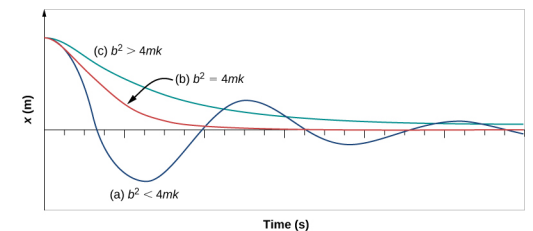
\includegraphics[width=0.75\linewidth]{images/damped-oscillator-three-cases.png}
    \caption{Graphs of the three cases solutions}
    \label{fig:damped-oscillator-three-cases}
\end{figure}

As we have seen above, usually in real life, our $b$ is relatively small, so we often encounter the \textbf{underdamped} oscillator. And to get a more intuitive feeling regarding the \textbf{underdamped} system, we can further manipulate our solution \ref{eq:damped-oscilation-complex-roots} by first writing out the two complex roots $\lambda$ \footnote{Here our $b$ is very small and to make the term under the $\sqrt{\cdots}$ always positive, we change the order from $(\frac{b}{2m})^2-\frac{k}{m}$ to $\frac{k}{m}-(\frac{b}{2m})^2$}
\begin{equation}
    \lambda=-\frac{b}{2m}\pm i\sqrt{\frac{k}{m}-(\frac{b}{2m})^2}
\end{equation}
Let's denote $\gamma=\frac{b}{2m},\omega=\sqrt{\frac{k}{m}-(\frac{b}{2m})^2}$. Then our solution becomes
\begin{equation}
    x(t)=c_1e^{-\gamma t}\cos \omega t+c_2e^{-\gamma t}\sin \omega t
\end{equation}
Then, use the auxiliary angle formula to simplify our result,
\begin{equation}
    x(t)=A_0e^{-\gamma t}\cos(\omega t+\varphi), \text{where }A_0=\sqrt{c_1^2+c_2^2},\varphi=\arctan\frac{c_2}{c_1}
\end{equation}
The significance of this solution is that now we know that in our \textbf{underdamped} oscillation system, how our new angular frequency $\omega$ and amplitude will change as the constant $b$ changes.

Notice that in the SHM without any damping force, the angular frequency $\omega_0=\sqrt{\frac{k}{m}}$. So, if our $b$ is very small, we can see that $\omega\approx\omega_0$, so means the angular frequency won't change much but the amplitude will slowly decrease. As shown below
\begin{figure}[h]
    \centering
    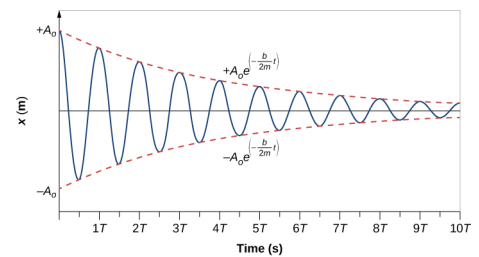
\includegraphics[width=0.75\linewidth]{images/underdamped-oscillator-example.png}
    \caption{Underdamped Oscillator Example}
    \label{fig:underdamped-oscillator-example}
\end{figure}
\end{document}